% ----------------------------------------------------------- %
\chapter{Comparative evaluation of algorithms and data strategies for cancer driver gene prediction}
\label{sec:results:comparative_evaluation}


In this chapter, we present and discuss a series of experiments designed to evaluate and compare various methodological strategies for predicting CDGs. Specifically, we focus on three decision levels: (i) the types of features used to describe genes (\ie, instances) for the prediction task, (ii) the strategies employed to address class imbalance, and (iii) the specific algorithm used for CDG prediction. In the latter, we include a comparative analysis between two classes of learning algorithms, traditional (\ie ``shallow'') ML algorithms and graph neural networks, to better understand the potential benefits of using graph-based learning for discovering CDGs. 


The following sections present the experimental setup and our results for this set of experiments. Our discussion will be oriented towards five main research questions:
\begin{itemize}
  \item \textit{RQ1} -- How does the choice of omics data used as node features impact the predictive performance of GNNs?
  \item \textit{RQ2} -- Can GNNs benefit from the inclusion of node centrality measures as node features?
  \item \textit{RQ3} -- What is the best strategy to handle class imbalance in the node prediction problem addressed?
  \item \textit{RQ4} -- How do traditional ML algorithms compare to GNNs when applied to the same omics data?
  \item \textit{RQ5} -- Which graph neural network model performs best for CDG prediction?
\end{itemize}

We conducted the analyses described in this chapter using the three smallest PPI networks presented in Section \ref{sec:materials_methods:ppinets}, namely HPRD, MULTINET, and IREF, due to the high computational costs involved. In total, we carried out 468 experiments testing variations in terms of features, algorithms, class imbalance strategies, and networks. For the sake of brevity, we focus our comparison mainly on the performance of the test set, and we present only the most meaningful results in this chapter. However, additional results for these experiments can be found in Appendix \ref{sec:appendix_cap5}, specifically in Tables \ref{tab:completa_hprd}, \ref{tab:completa_multinet}, and \ref{tab:completa_iref} for GNNs, and Tables \ref{tab:completa_trad_hprd}, \ref{tab:completa_trad_multinet}, and  \ref{tab:completa_trad_iref} and Figure~\ref{fig:aucpr_roc_nn} for traditional ML algorithms. 

\section{Experiments setup}

To ensure a fair comparison between the selected GNN algorithms, we maintained fixed hyperparameter values across all experiments described in this chapter. This approach allowed us to focus on comparing the impact of other decisions related to the methodology employed in model development. Table \ref{tab:param_comparison} shows the hyperparameter configuration for the three GNN algorithms, with most of the values defined as default by the StellarGraph library. The cross-entropy loss function was used in all experiments unless loss function variations are mentioned in the text, \eg when assessing the class imbalance solutions. Furthermore, since we used the same Python library to train GNN models in our experiments (as described in Chapter \ref{sec:materials_methods}), the data structure used was the same for all algorithms, making performance comparisons more straightforward. 



The models based on SVM, RF, and GBT were built using the Scikit-learn library \cite{scikit-learn} and the ANN was trained using the Keras library \cite{chollet2015keras}. For the ANN, we configured the hyperparameters similar to the values presented in Table~\ref{tab:param_comparison}. We used two hidden layers with 64 neurons in each, the cross-entropy loss function, and a dropout rate and learning rate of 0.01 and 0.001, respectively. The hyperparameters for the remaining algorithms (\ie RF, GBT, and SVM), were kept as the default values provided by the Scikit-learn library (version 1.1.1).


Model evaluation was conducted as explained in Chapter \ref{sec:materials_methods}, applying the Holdout method followed by 5-fold CV in the training data for GNNs, and using a 5-fold CV over the complete dataset for traditional ML algorithms. Although accuracy and AUC-ROC were collected through the experiments, we concentrate our discussion in the AUC-PR metric, as it represents a better compromise for evaluating problems with class imbalance in which the other metrics tend to be highly optimistic.

\begin{table}[!th]
\centering
\caption{Hyperparameters configuration used for GNNs in the comparative evaluation experiments. \label{tab:param_comparison}}
\resizebox{0.9\textwidth}{!}{
\begin{tabular}{lccc}
\hline
\multicolumn{1}{c}{Hyperparameter}   & \multicolumn{3}{c}{Algorithm}                 \\ \hline
                                      & GAT           & GCN           & GraphSAGE     \\ \cline{2-4} 
Number of layers                      & 2             & 2             & 2             \\
Number of units on each layer & 64            & 64            & 64            \\
Activation function                   & ReLU          & ReLU          & ReLU          \\
Loss function                         & Cross-entropy & Cross-entropy & Cross-entropy \\
Dropout rate                              & 0.01          & 0.01          & 0.01          \\
Learning rate                         & 0.001         & 0.001         & 0.001         \\
Number of epochs                      & 300           & 300           & 300           \\
Attention heads                       & 8             & -             & -             \\
Attention dropout                     & 0.01          & -             & -             \\
Batch size                            & 1             & 1             & 50            \\
Number of samples per layer           & -             & -             & 10 and 5      \\ \hline
\end{tabular}}
\end{table}



\section{Results}

\subsection{How does the choice of omics data used as node features impact the predictive performance of GNNs?}
\label{sec:results:comparative_evaluation:rq1}

Similarly to traditional ML algorithms, GNNs can leverage the information provided by node feature vectors to learn patterns associated to CDGs.  By integrating this information with the local structure of the nodes in the graph, the GNN learns to predict their labels. Therefore, it is reasonable to assume that the use of different types of omics data as node feature vectors may impact on the performance of the model.

To evaluate the effects of applying different types of omics data as node features on the performance of GNN models, we carried out five experiments with each of the smallest PPI networks (\ie HPRD, MULTINET, and IREF). First, we analyzed the model performance using a single type of omics data (\eg Mutations, CNA, DNA Methylation, or Gene expression) as node feature vectors during training. Next, we trained models concatenating the four types of omics data as node features, which is known as a multi-omics approach. We note that these experiments used the traditional cross-entropy loss function, thus, they do not address the issue of class imbalance.

Table \ref{tab:results1_comparison} summarizes the results for the AUC-PR metric for the test set. We highlight in boldface the best results for each algorithm and PPI network. It is worth noting that the overall performance of all GNN models falls short of what is expected from a good classifier. The low AUC-PR values suggest that the models are not performing well in correctly identifying all true CDGs and avoiding false positive predictions, which means classifying a gene as a cancer driver when it is not. Nevertheless, given the significant class imbalance in our dataset, such difficulty is expected, and the performance metrics still provide a basis for comparison.
 

\begin{table}[!ht]
\centering
\caption{AUC-PR performance comparison among GNNs for variations of types of omics data used as node features. \label{tab:results1_comparison}}
%\resizebox{0.7\textwidth}{!}{
\begin{tabular}{lcccc}
\hline
\multicolumn{1}{c}{Features} & PPI Network & \multicolumn{3}{c}{Algorithm}                       \\ \hline
                             &         & GAT             & GCN             & GraphSAGE       \\ \cline{3-5} 
Mutations                    &      \multirow{5}{*}{HPRD}       & 0.3565          & 0.4470          & \textbf{0.4089} \\
CNA                          &             & 0.2761          & 0.3992          & 0.3134          \\
DNA Methylation              &             & \textbf{0.3844} & 0.3708          & 0.2402          \\
Gene Expression              &             & 0.2806          & 0.2967          & 0.2397          \\
Multi-Omics                  &             & 0.3258          & \textbf{0.4984} & 0.3317          \\
                             &     &                 &                 &                 \\
Mutations                    &  \multirow{5}{*}{MULTINET}           & 0.2142          & 0.3523          & \textbf{0.3842} \\
CNA                          &             & \textbf{0.2865} & 0.3277          & 0.1996          \\
DNA Methylation              &             & 0.2219          & 0.3185          & 0.1770          \\
Gene Expression              &             & 0.2562          & 0.2506          & 0.1981          \\
Multi-Omics                  &             & 0.2182          & \textbf{0.3839} & 0.2671          \\
                             &        &                 &                 &                 \\
Mutations                    & \multirow{5}{*}{IREF}            & 0.2606          & \textbf{0.4344} & \textbf{0.3550} \\
CNA                          &             & 0.3027          & 0.2844          & 0.2036          \\
DNA Methylation              &             & \textbf{0.3088} & 0.2509          & 0.1482          \\
Gene Expression              &             & 0.2211          & 0.2699          & 0.1850          \\
Multi-Omics                  &             & 0.2144          & 0.4315          & 0.2001          \\ \hline
\end{tabular}%}
\end{table}

Our experiments showed that the choice of node feature vector can have a significant impact on the performance of GNN models. For example, in the HPRD PPI network, performance ranged from 0.2761 (using \textit{CNA} node features) to 0.3844 (using \textit{DNA Methylation}) for GAT, from 0.2967 (using \textit{Gene Expression}) to 0.4984 (using \textit{Multi-omics}) for GCN, and from 0.2397 (using \textit{Gene Expression}) to 0.4089 (using \textit{Mutations}) for GraphSage. GraphSage consistently showed the largest performance variations between minimum and maximum values across the three PPI networks (HPRD: 70.58\%, MULTINET: 117.06\%, and IREF: 139.54\%), while GAT showed the smallest (HPRD: 39.22\%, MULTINET: 33.75\%, and IREF: 44.02\%), indicating that GraphSage is more sensitive to changes in node features than GAT and GCN in our domain.

Additionally, the ranking of feature types based on performance is not consistent across all networks and algorithms. For instance, while \textit{Mutation} yielded the highest performance in four out of the nine combinations of PPI network and GNN algorithm,  \textit{Multi-omics} and \textit{DNA methylation} achieved the best performance in two combinations each. \textit{CNA}, on the other hand, was the top-performing feature set in only one combination. This result is biologically plausible, since DNA mutations are the primary cause of most cancers. Nonetheless, integrating the four types of omics in the multi-omics approach still seemed advantageous as it was able to improve performance in some cases, especially for the GCN algorithm. Thus, for the next experiment, we select the multi-omics strategy as our default configuration for the node features vector.



\subsection{Can GNNs benefit from the inclusion of node centrality measures as node features?}
\label{sec:results:comparative_evaluation:rq2}

Node centrality measures, such as degree and betweenness,  %(see Section \ref{sec:deep_and_gnns} for details),
are commonly employed as handcrafted graph features for ML approaches in disease gene prediction. This was the traditional approach to explore the information contained in biological networks (e.g., PPI networks) in node prediction tasks before the advent of graph-based learning algorithms \cite{ata2021recent}. Given that node centrality measures were relatively successful in capturing the global and local graph structure of nodes in previous efforts, we aimed to investigate whether they can increase model reliability and improve performance metrics when used as features along with multi-omics data.


We extracted four node centrality measures - degree, betweenness, closeness, and clustering coefficient (see Section \ref{sec:deep_and_gnns} for definitions) - from each of the PPI networks using the igraph package \cite{igraphpackage}. These centrality measures were used exclusively as additional features for the PPI network from which they were computed since they are node features that rely on the graph structure. We then conducted a new round of model training and evaluation using a node feature vector composed of multi-omics data and centrality measures.


\begin{figure*}[!bh]
    \centering
      \caption{Analysis of the impact of the inclusion of centrality measures as node features in the performance of GNNs.}
    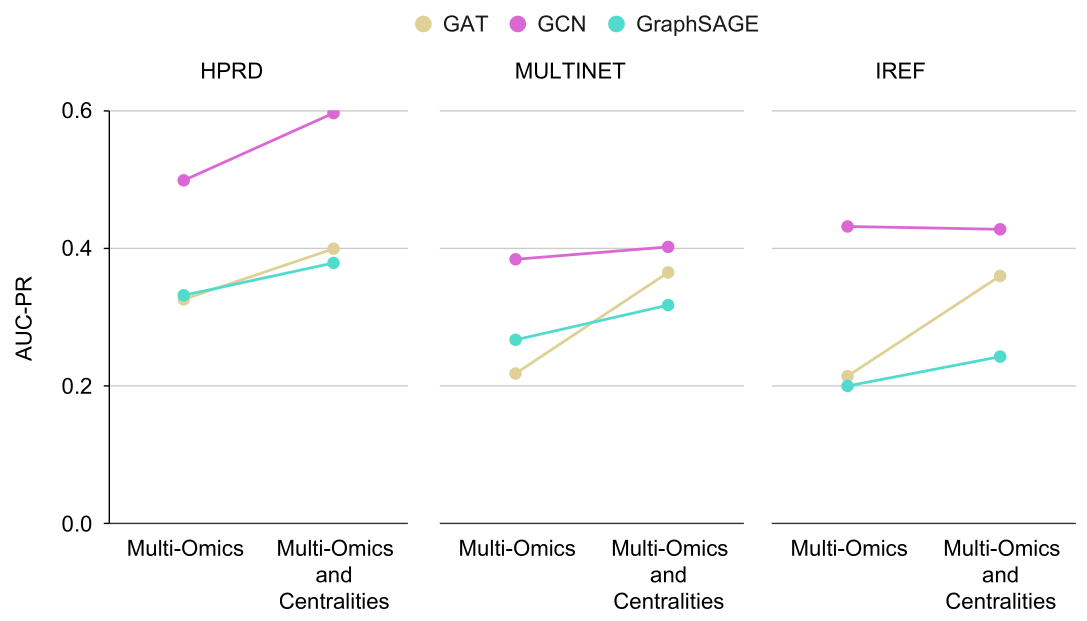
\includegraphics[width=0.95\textwidth]{images/ilustracoes/omics_completo.png}
    \legend{Source: Prepared by the author}
    \label{fig:omics_completo}

\end{figure*}

Figure~\ref{fig:omics_completo} shows the results of this experiment for the test set, compared against the results when considering only multi-omics features (Section~\ref{sec:results:comparative_evaluation:rq1}). We observed that centrality measures provided important information for training the model since they improved the performance in most scenarios. The only exception was the GCN model for the IREF network, which did not benefit from the additional features. The predictive performance increased up to 67.81\% for the GAT model applied to the IREF network. In general, the GAT model was the most benefited when adding centrality measures to the node features vector, although the GCN model also significantly improved the predictive performance after the inclusion of centrality features in the HPRD network. 

Whereas Figure~\ref{fig:omics_completo} presents the results for the independent test set, which is our main interest for performance comparison, we also provide the learning curves for the HPRD network when using multi-omics and centralities as node features in Figure~\ref{fig:fullfeatset_epochs_hprd} (the same analyses can be seen for MULTINET and IREF networks in the Appendix~\ref{sec:appendix_cap5}, Figures \ref{fig:aucpr_roc_multinet} and \ref{fig:aucpr_roc_iref}). 
These figures allow us to evaluate the training and validation performance history of the algorithms through 300 epochs. Values represent the mean and standard deviation across 5-fold CV. We note that GAT (Figure~\ref{fig:gat_aucpr_roc_hprd}) and GraphSage (Figure~\ref{fig:sage_aucpr_roc_hprd}) tend to quickly overfit in the first 50 epochs when using default hyperparameters. Moreover, GAT shows the highest performance variation among the five repetitions.


\begin{figure*}[!ht]
\centering

%\caption{Training and validation for the HPRD network in GAT (a), GCN (b) and GraphSAGE (c) using 300 epochs and AUC-PR and AUC-ROC as performance metrics}
\caption{Training and validation performance for the HPRD network in (a) GAT, (b) GCN, and (c) GraphSAGE in terms of AUC-PR (left column) and AUC-ROC values (right column).\label{fig:fullfeatset_epochs_hprd}}
   \subfloat[GAT \label{fig:gat_aucpr_roc_hprd}]{%
      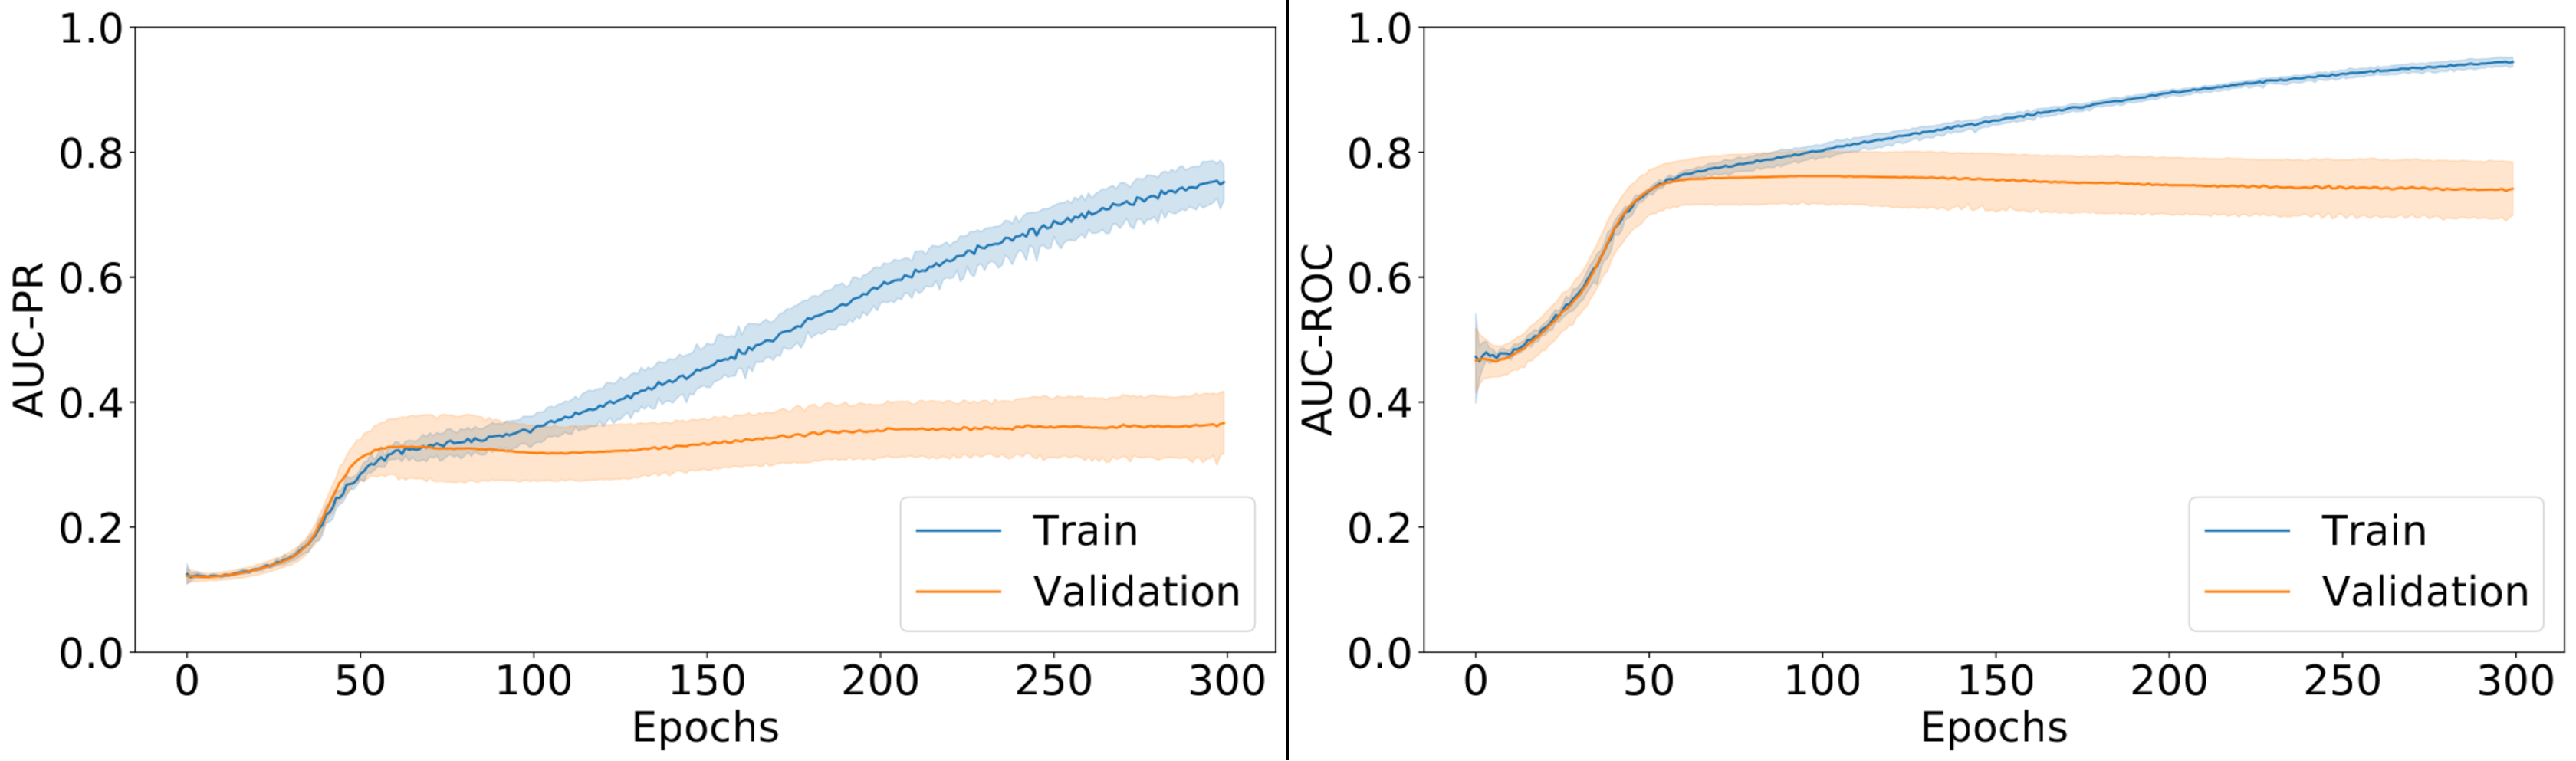
\includegraphics[width=\textwidth]{images/results/aucpr_roc_gat.pdf}}
\hspace{\fill}
   \subfloat[GCN \label{fig:gcn_aucpr_roc_hprd} ]{%
      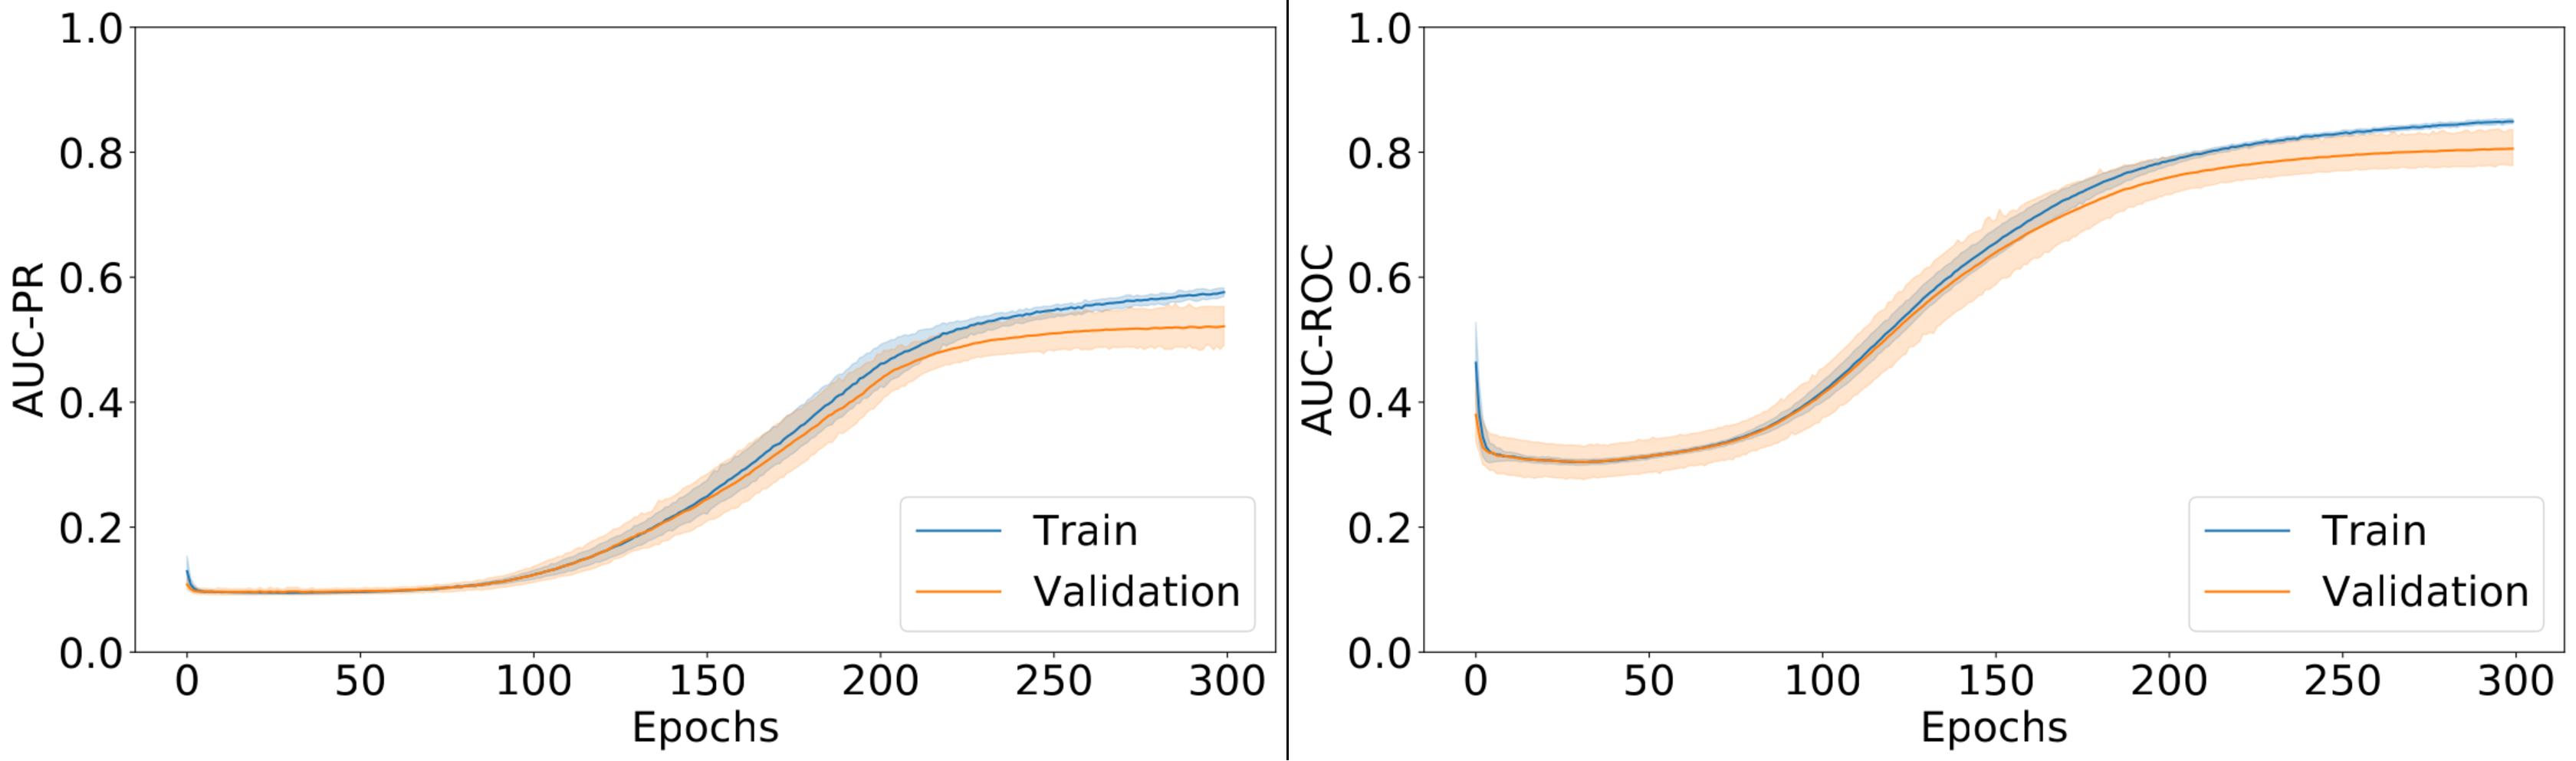
\includegraphics[width=\textwidth]{images/results/aucpr_roc_gcn.pdf}}
\hspace{\fill}
   \subfloat[GraphSAGE \label{fig:sage_aucpr_roc_hprd}]{%
      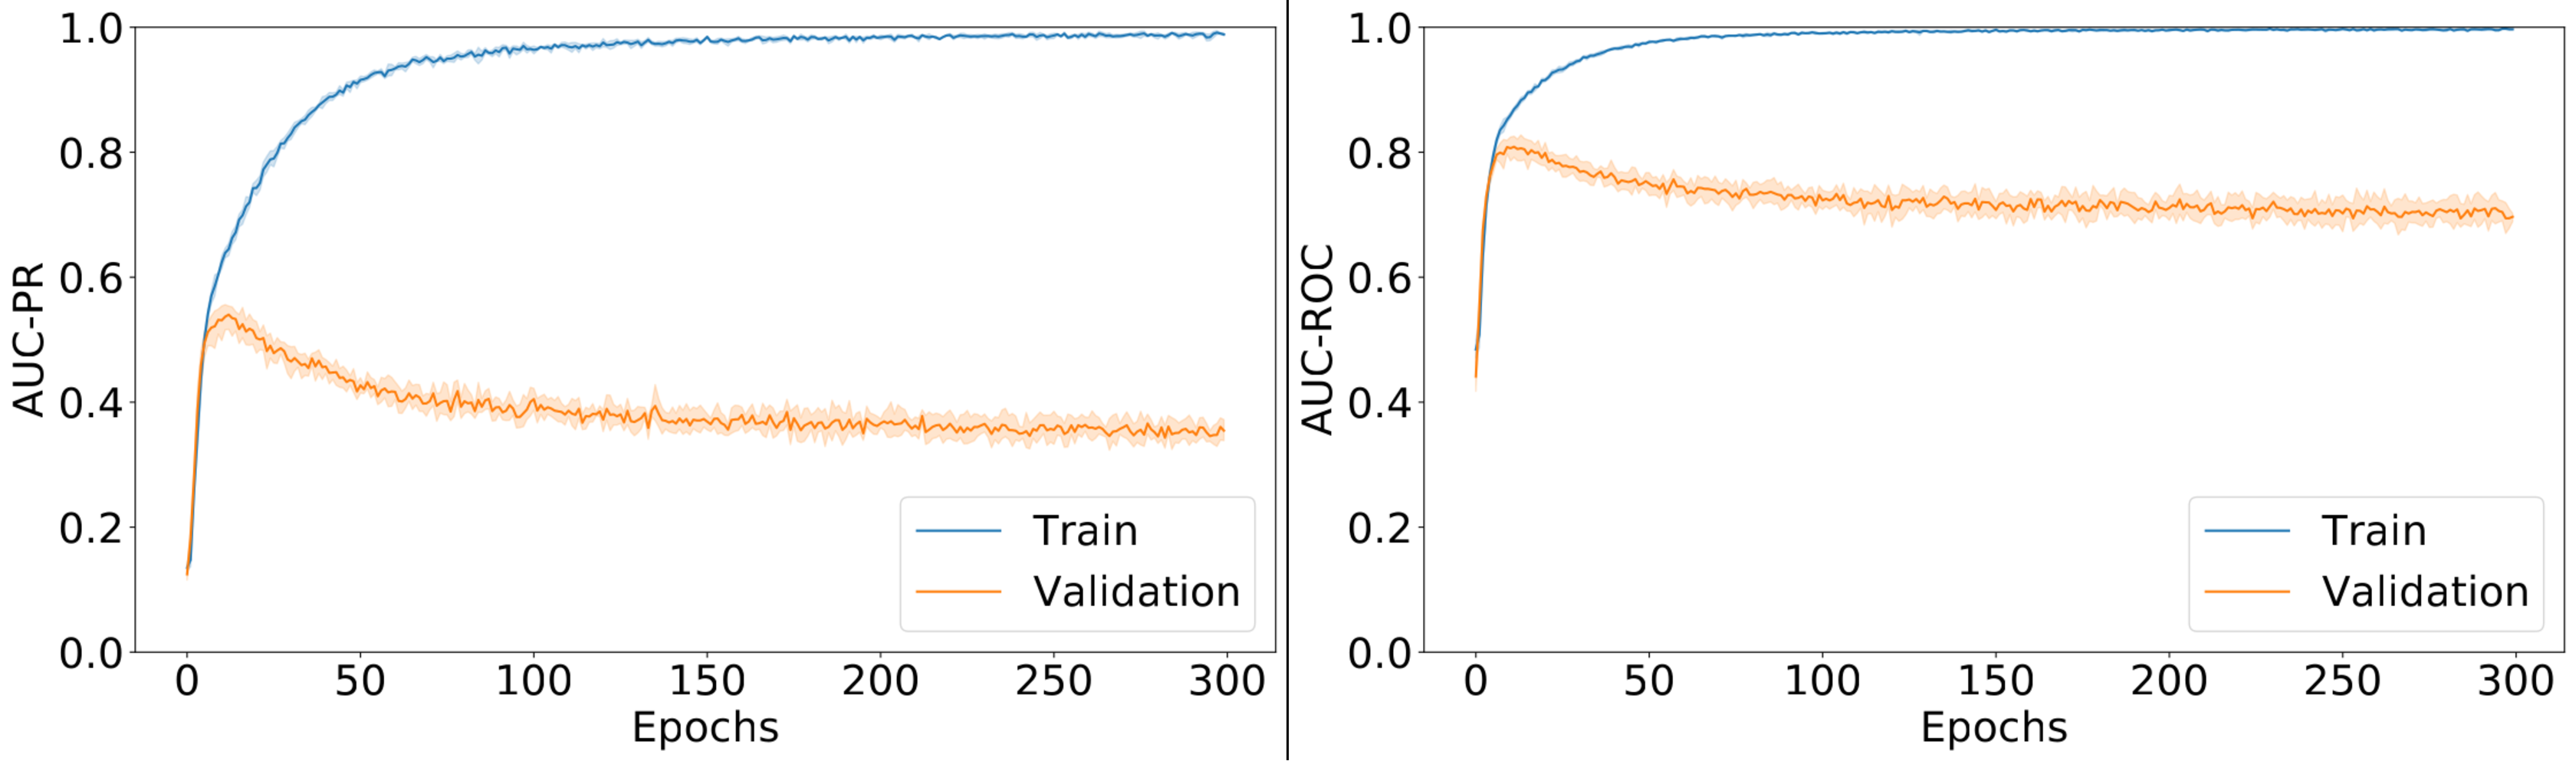
\includegraphics[width=\textwidth]{images/results/aucpr_roc_sage.pdf}}\\
\legend{Source: Prepared by the author}
\label{fig:aucpr_roc_hprd}
\end{figure*}

Another interesting point in Figure~\ref{fig:fullfeatset_epochs_hprd} is that the ROC curves (right column) are all shifted upwards compared to the PR curves (left column). This means that the model evaluation through the AUC-ROC metric suggests higher predictive performance. However, this is an artifact of our dataset, which contains a low proportion of instances in the positive class (\ie true CDGs). 

To better illustrate this issue and reinforce our choice to focus the comparative analysis on the AUC-PR values, we provide a direct comparison among accuracy, AUC-ROC, and AUC-PR for the test set (Table~\ref{tab:results1_metrics_comparison}). We observed that accuracy and AUC-ROC are always higher than AUC-PR for every combination of GNN algorithm and PPI network. While the AUC-PR values range from 0.2427 to 0.5960 in these experiments, accuracy varies between 0.8289 and 0.9213, and AUC-ROC varies between 0.6629 and 0.8453. Finally, given that the use of centrality measures as node features improve the predictive performance for graph-based learning algorithms, from this point forward, we will always use the node feature vector composed of multi-omics data and centrality measures as the default feature set.


\begin{table}[!th]
\centering
\caption{Different performance metrics for predictions on the test set using a combination of multi-omics and centrality measures as node features. \label{tab:results1_metrics_comparison}}
\begin{tabular}{clccc}
\hline
\multicolumn{1}{l}{Algorithm} & PPI Network & \multicolumn{3}{c}{Performance metric} \\ \hline
\multicolumn{1}{l}{}          &             & Accuracy     & AUC-ROC     & AUC-PR    \\ \cline{3-5} 
\multirow{3}{*}{GAT}          & HPRD        & 0.8580       & 0.7969      & 0.3992    \\
                              & MULTINET    & 0.9043       & 0.8312      & 0.3648    \\
                              & IREF        & 0.9120       & 0.8453      & 0.3598    \\
\multicolumn{1}{l}{}          &             &              &             &           \\
\multirow{3}{*}{GCN}          & HPRD        & 0.8889       & 0.8418      & 0.5960    \\
                              & MULTINET    & 0.9123       & 0.8162      & 0.4019    \\
                              & IREF        & 0.9213       & 0.8246      & 0.4274    \\
\multicolumn{1}{l}{}          &             &              &             &           \\
\multirow{3}{*}{GraphSAGE}    & HPRD        & 0.8289       & 0.7132      & 0.3786    \\
                              & MULTINET    & 0.9011       & 0.7201      & 0.3174    \\
                              & IREF        & 0.8827       & 0.6629      & 0.2427    \\ \hline
\end{tabular}
\end{table}

\subsection{What is the best strategy to handle class imbalance in the node prediction problem addressed?}
\label{sec:results:comparative_evaluation:rq3}

Class imbalance is a recurring problem when working with cancer genomics and cancer driver prediction, as the target factor, either a true driver mutation or a true CDG, is always the most rare phenomenon when compared to passenger mutations or neutral genes. As noted in Chapter \ref{sec:related_works}, other authors also face this inherent obstacle, although only a few reviewed papers clearly discuss the strategy adopted to address this issue.


\begin{table}[!bh]
\centering
\caption{AUC-PR peformance comparison between strategies to address the class imbalance issue. The values refer to predictive performance on the test set. \label{tab:results2_comparison}}
\begin{tabular}{lcccc}
\hline
\multicolumn{1}{c}{Strategy} & PPI Network & \multicolumn{3}{c}{Algorithm}                       \\ \hline
                                  &        & GAT             & GCN             & GraphSAGE       \\ \cline{3-5} 
Cross-entropy                     & \multirow{6}{*}{HPRD}            & 0.3992          & \textbf{0.5960} & 0.3786          \\
Undersampling                     &             & 0.3275          & 0.5479          & 0.3332          \\
Balanced cross-entropy ($\alpha$=0.85) &             & \textbf{0.4215} & 0.5918          & 0.4069          \\
Focal loss ($\gamma$=0.5; $\alpha$=0.50)        &             & 0.3873          & 0.5235          & 0.4230          \\
Focal loss ($\gamma$=1; $\alpha$=0.25)          &             & 0.3581          & 0.5756          & 0.3985          \\
Focal loss ($\gamma$=2; $\alpha$=0.25)          &             & 0.3792          & 0.5583          & \textbf{0.4480} \\
                                  &     &                 &                 &                 \\
Cross-entropy                     & \multirow{6}{*}{MULTINET}            & 0.3648          & 0.4019          & 0.3174          \\
Undersampling                     &             & 0.2817          & 0.4521          & 0.2188          \\
Balanced cross-entropy ($\alpha$=0.85) &             & 0.3551          & \textbf{0.4661} & \textbf{0.3929} \\
Focal loss ($\gamma$=0.5; $\alpha$=0.50)        &             & \textbf{0.4143} & 0.4177          & 0.3264          \\
Focal loss ($\gamma$=1; $\alpha$=0.25)          &             & 0.3363          & 0.2978          & 0.3196          \\
Focal loss ($\gamma$=2; $\alpha$=0.25)          &             & 0.2753          & 0.4481          & 0.3822          \\
                                  &        &                 &                 &                 \\
Cross-entropy                     & \multirow{6}{*}{IREF}            & 0.3598          & 0.4274          & 0.2427          \\
Undersampling                     &             & 0.1714          & 0.4384          & 0.1887          \\
Balanced cross-entropy ($\alpha$=0.85) &             & 0.3135          & \textbf{0.4841} & \textbf{0.3013} \\
Focal loss ($\gamma$=0.5; $\alpha$=0.50)        &             & 0.3546          & 0.4664          & 0.2296          \\
Focal loss ($\gamma$=1; $\alpha$=0.25)          &             & 0.2977          & 0.3776          & 0.2832          \\
Focal loss ($\gamma$=2; $\alpha$=0.25)          &             & \textbf{0.3917} & 0.4488          & 0.2928          \\ \hline
\end{tabular}
\end{table}


In Section \ref{sec:background_ClassImbalance}, we presented the theoretical foundation for most common strategies to deal with class imbalance, which we experimentally compare in the current section: Random Undersampling, Balanced Cross-entropy, and Focal Loss. For each GNN algorithm and PPI network, we applied five different strategies to mitigate the class imbalance among positive and negative examples of CDGs. Besides Random Undersampling and Balanced Cross-entropy, we selected three variations of the Focal Loss function from the original article \cite{lin2017focal}, which presents a series of experiments and arrives at a set of best combinations for the hyperparameters $\gamma$ and $\alpha$. We used $\gamma$ = 0.5 and $\alpha$ = 0.50, $\gamma$ = 1 and $\alpha$ = 0.25, and $\gamma$ = 2 and $\alpha$ = 0.25. We note that the Balanced Cross-Entropy resembles a Focal loss function with $\gamma = 0$ and with the $\alpha$ parameter indicating the weight to balance the importance of positive/negative instances (here, we adopted  $\alpha = 0.85$). The Cross-entropy cost function was used in two moments: in the initial experiments conducted previously (considered as our ``baseline'') and in the scenario where the Random Undersampling technique is applied to data. Table \ref{tab:results2_comparison} presents the results of our experiments comparing strategies to deal with class imbalance. The best results for each algorithm and PPI network are highlighted in boldface.



 Overall, we observed performance improvements in most cases where class imbalance correction was carried out. Balanced Cross-Entropy yielded the most promising results, while the undersampling strategy was generally less effective. Although the results are still below the desired level of predictive performance, they show potential for further improvement through hyperparamenter optimization in the case of Balanced Cross-Entropy and Focal Loss. Since the Balanced Cross-Entropy is a special case of a Focal Loss, we defined Focal Loss as the most promising approach to handle class imbalance in our domain. 


\subsection{How do traditional ML algorithms compare to GNNs when applied to the same omics data?}
\label{sec:results:comparative_evaluation:rq4}

As part of our investigation, we aimed to understand the potential benefits of using the full network structure through graph-based learning methods compared to relying solely on handcrafted features such as omics data and centrality measures for model learning. To this end, we conducted a series of experiments with four traditional ML algorithms widely used in the bioinformatics domain: SVM, Random Forests, Gradient Boosting Trees, and Artificial Neural Networks. For more information on the theoretical background, please refer to Chapter \ref{sec:background}.




\begin{table}[!th]
\centering
\caption{AUC-PR peformance comparison among traditional ML algorithms and variations in the omics data used as features. \label{tab:results3_comparison}}
\begin{tabular}{lccccc}
\hline
\multicolumn{1}{c}{Features} & PPI Network                  & \multicolumn{4}{c}{Algorithm}                                                                                                                                                                \\ \hline
                             & \multicolumn{1}{c}{}     & SVM    & \begin{tabular}[c]{@{}c@{}}RF\end{tabular} & \begin{tabular}[c]{@{}c@{}}GBT\end{tabular} & \begin{tabular}[c]{@{}c@{}}ANN\end{tabular} \\ \cline{3-6} 
Mutations                    &      \multirow{5}{*}{HPRD}                         & 0.3272 & 0.3664                                                   & \textbf{0.3753}                                              & 0.2252                                                    \\
CNA                          &                              & 0.1950 & 0.1702                                                   & 0.1846                                                       & 0.1619                                                    \\
DNA Methylation              &                              & 0.1435 & 0.1519                                                   & 0.1487                                                       & 0.1324                                                    \\
Gene Expression              &                              & 0.1368 & 0.1559                                                   & 0.1564                                                       & 0.1563                                                    \\
Multi-Omics                  &                              & 0.2595 & 0.3566                                                   & 0.3565                                                       & 0.2119                                                    \\
                             & \multicolumn{1}{c}{} &        &                                                          &                                                              &                                                           \\
Mutations                    &     \multirow{5}{*}{MULTINET}                          & 0.2819 & 0.3066                                                   & \textbf{0.3212}                                              & 0.1726                                                    \\
CNA                          &                              & 0.1247 & 0.1136                                                   & 0.1169                                                       & 0.1220                                                    \\
DNA Methylation              &                              & 0.0951 & 0.1122                                                   & 0.1089                                                       & 0.0853                                                    \\
Gene Expression              &                              & 0.0997 & 0.1071                                                   & 0.1151                                                       & 0.0946                                                    \\
Multi-Omics                  &                              & 0.2025 & 0.2976                                                   & 0.3066                                                       & 0.1614                                                    \\
                             &   &        &                                                          &                                                              &                                                           \\
Mutations                    &      \multirow{5}{*}{IREF}                          & 0.2598 & 0.2929                                                   & \textbf{0.3087}                                              & 0.1848                                                    \\
CNA                          &                              & 0.1204 & 0.1201                                                   & 0.1268                                                       & 0.1165                                                    \\
DNA Methylation              &                              & 0.0969 & 0.1023                                                   & 0.1044                                                       & 0.1081                                                    \\
Gene Expression              &                              & 0.0906 & 0.1016                                                   & 0.1077                                                       & 0.0981                                                    \\
Multi-Omics                  &                              & 0.1958 & 0.2869                                                   & 0.3029                                                       & 0.1519                                                    \\ \hline
\end{tabular}
\end{table}

For the traditional ML algorithms, we had a conventional classification task in which the algorithm was only provided with a dataframe containing instances (\ie genes) with their features vector and corresponding label. The structure of the PPI network was not used when the features were based solely on omics data. Therefore, the predictive performance was entirely associated with the informative power of omics data. Nevertheless, we performed experiments for each PPI network since the set of genes analyzed differed among networks. To ensure consistency, we kept the hyperparameters constant through all experiments and evaluated the impact of omics levels on each algorithm.

Table \ref{tab:results3_comparison} summarizes the results for the test set. The best performance per PPI network is highlighted in boldface, and the values refer to the average performance across 5-fold CV. The traditional ML algorithms performed better on mutation data, but the overall performance of these models was worse than those achieved by GNN algorithms. Among the four traditional ML algorithms applied, GBT was the top-performing one for all PPI networks, followed by RF. Multi-omics data was the second-best feature set for all PPI networks.

We also assessed the effect of using class weights during training to adjust the cost of misclassifications and avoid concentrating the learning on the majority class, similar to the experiments with GNNs. However, these experiments did not yield any significant results since most of the models did not exceed the standard performance presented in Table \ref{tab:results3_comparison} upon class imbalance mitigation with class weights. Therefore, we do not report these results here.


Finally, we assessed the impact of incorporating node centrality measures as features in traditional ML algorithms, inspired by the promising results achieved with GNNs. We used the multi-omics features vector as our baseline and added measures for node degree, betweenness, closeness, and clustering coefficient for each PPI network. The results presented in Figure \ref{fig:centralidades_tradicionais} demonstrate that the inclusion of centrality measures as an extra source of information improved the performance of all models, surpassing the results obtained with individual omics data or their combination (i.e., multi-omics). We can also clearly visualize that the magnitude of performance change upon addition of centrality measures was greater for traditional algorithms than for GNNs (Figure~\ref{fig:omics_completo} ), which is expected, since GNNs by definition already have information about the graph (\ie PPI network) in the learning process. Another interesting observation is that the decision tree-based algorithm had a very close  performance in this prediction task, and also very similar behavior with the inclusion of centrality features.

\begin{figure*}[!th]
    \centering
      \caption{Analysis of the impact of including node centrality measures as features in the traditional ML algorithms.}
    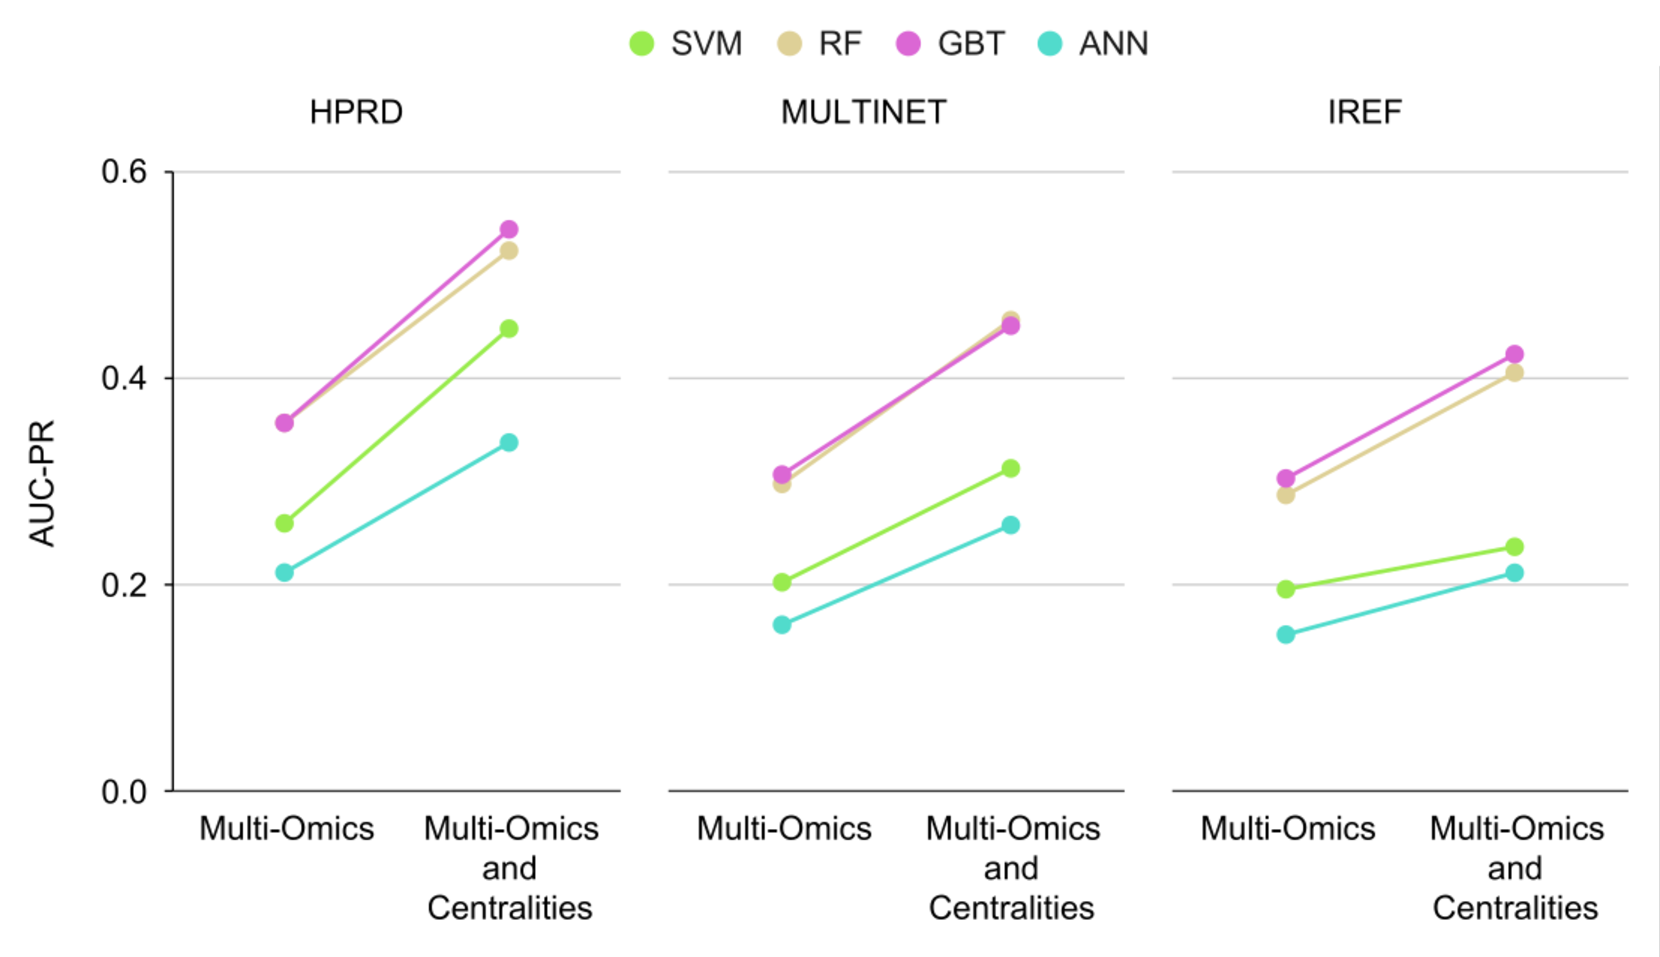
\includegraphics[width=0.95\textwidth]{images/ilustracoes/omics_completo_trad.pdf}
    \label{fig:centralidades_tradicionais}
\end{figure*}



After comparing the results of experiments using multi-omics data and node centralities among the best-performing traditional ML algorithm (\ie GBT) and GNNs, as depicted in Figure \ref{fig:comparacao_gnn_trad}, we can conclude that GBT had a competitive performance in relation to graph-based models. GBT achieved better results than GAT and GraphSAGE for all PPI networks. When we compared GCN and GBT, we noticed that GCN outperformed GBT in two of the analyzed networks, while GBT achieved the highest score among all the evaluated approaches for MULTINET. 

\begin{figure*}[!th]
    \centering
      \caption{Comparison between GNNs and GBT using multi-omics and node centralities as features.}
    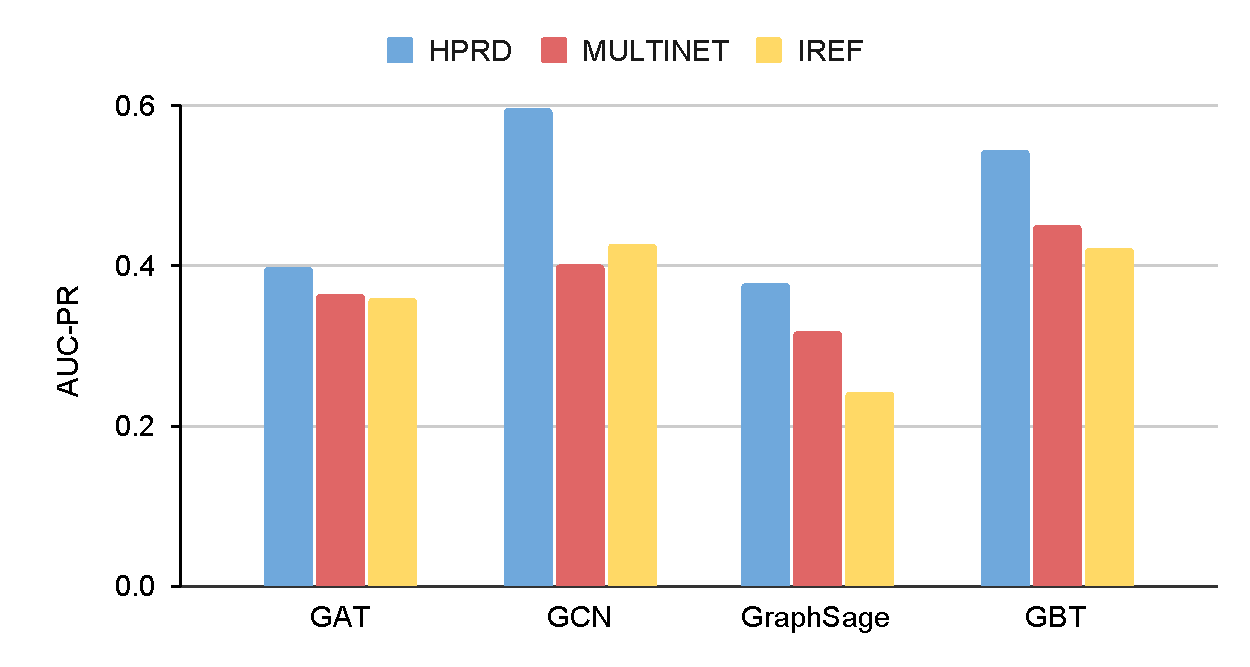
\includegraphics[width=0.85\textwidth]{images/ilustracoes/comparacao_gnn_trad.pdf}
    \label{fig:comparacao_gnn_trad}
\end{figure*}


Overall, our experiments indicate that the task of predicting CDGs is, in general, more challenging for traditional ML algorithms than for GNNs. However, traditional ML algorithms stand out in some cases, as in the use of tree-based methods with mutation data. Additionally, our analyses including centrality measures highlighted their relevance as a complement to multi-omics data. This was particularly evident in this set of experiments, where centralities played a significant role in enhancing the predictive performance obtained with multi-omics data for algorithms that learn from tabular data.
These observations underscore the importance of considering the network structure for CDG prediction and suggest that centralities may play a critical role in such scenarios.


\subsection{Which graph neural network algorithm performs best for CDG prediction?} 
\label{sec:results:comparative_evaluation:rq5}


The last and main question raised in this chapter refers to investigating which of the GNN algorithms is the most promising for the task of predicting CDGs. After conducting several exploratory experiments comparing various approaches, we aimed to select one algorithm for further development through a more detailed methodological process, including hyperparameter optimization, in an effort to improve its predictive performance for this task. 


\begin{figure}[hb!]
\centering
\caption{Test set cross entropy performance of (a) HPRD, (b) MULTINET, and (c) IREF networks.\label{fig:gnns_summary}}
 \subfloat[HPRD \label{fig:hprd_features_aucpr}]{%
      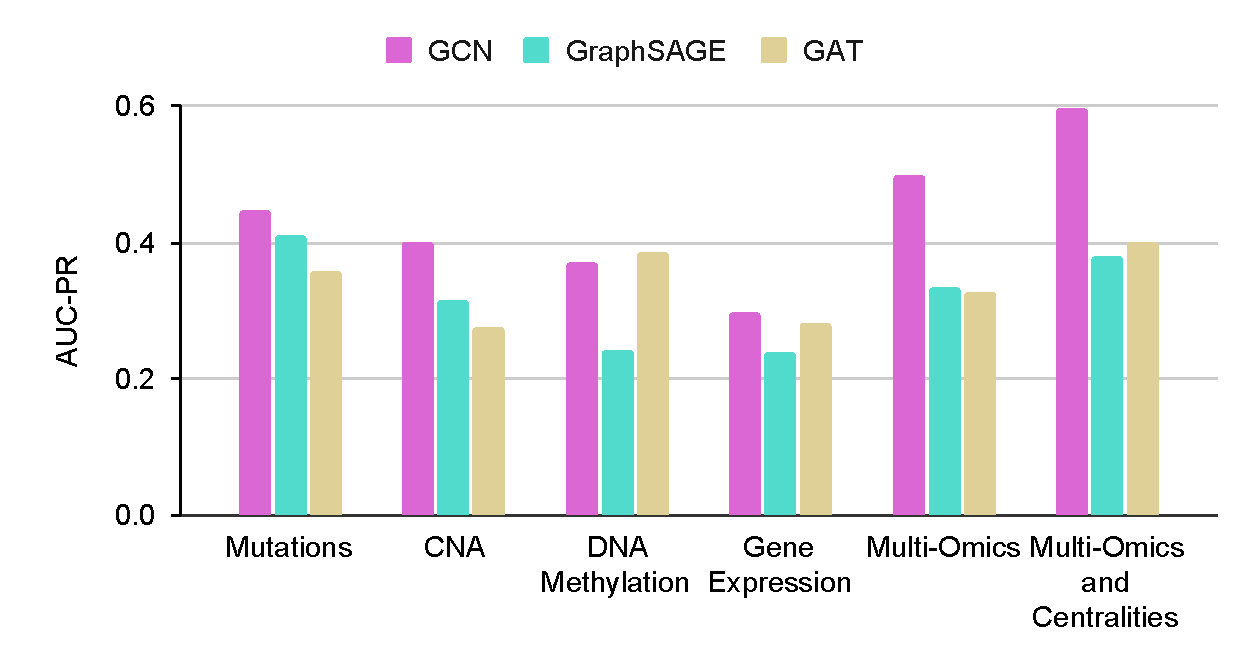
\includegraphics[width=0.80\textwidth]{images/ilustracoes/hprd_features_aucpr.pdf}}
      
   \subfloat[MULTINET \label{fig:multinet_features_aucpr}]{%
      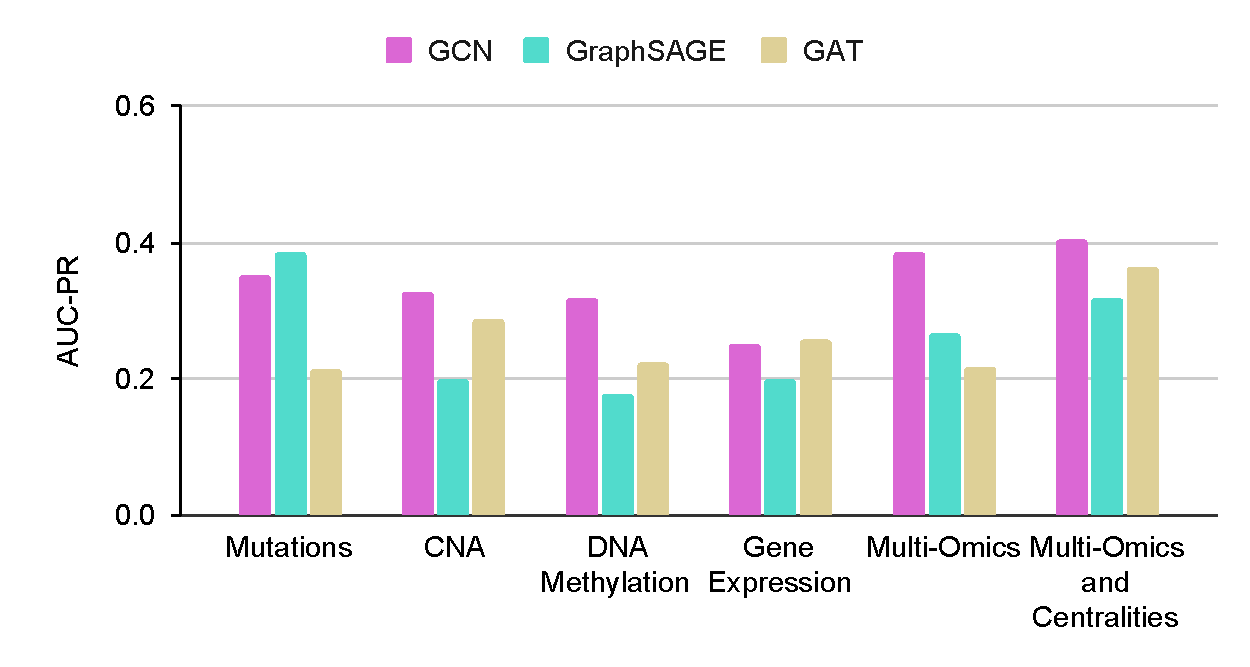
\includegraphics[width=0.80\textwidth]{images/apendice/multinet_features_aucpr.pdf}}
      
   \subfloat[IREF \label{fig:iref_features_aucpr}]{%
      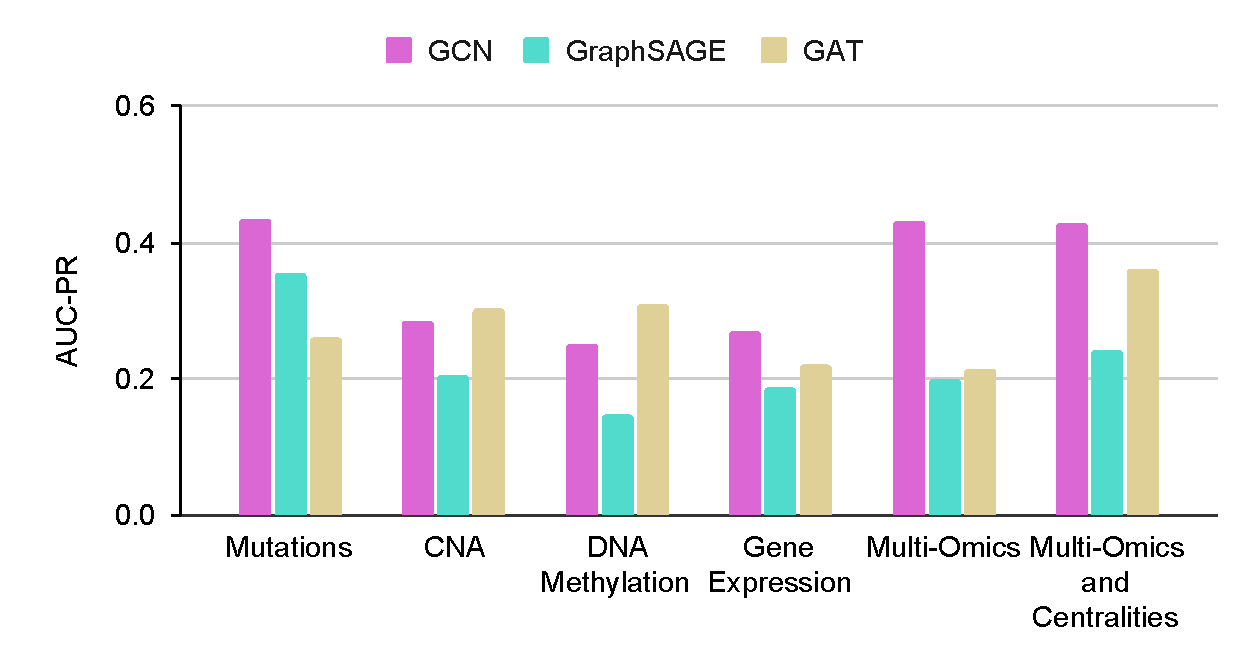
\includegraphics[width=0.80\textwidth]{images/apendice/iref_features_aucpr.pdf}}\\
\end{figure}




Figure \ref{fig:gnns_summary} provides a comparison of the test performance measures of the three evaluated GNN algorithms. Based on our analysis of these results, as well as the findings discussed in Sections \ref{sec:results:comparative_evaluation:rq1} to \ref{sec:results:comparative_evaluation:rq4} in this chapter, we concluded that GCN is the most promising algorithm for accurately predicting CDGs. GCN demonstrated superior performance in nearly all scenarios tested, in terms of both PPI networks and the composition of the node features vector. Additionally, the highest performance achieved in this experimental comparison was associated with the use of GCN in conjunction with multi-omics and centralities. Consequently, we have chosen the GCN model and the feature set comprising multi-omics and centrality measures as our standard approach for the learning algorithm and data representation. In the next chapter, we will provide a more in-depth investigation of this strategy, including efforts to optimize hyperparameters.




\section{Summary}

The primary focus of this chapter was to investigate the potential of GNN algorithms and distinct feature definition strategies for predicting CDGs.
A series of experiments were carried out to extract an understanding about how, in general, GNN algorithms perform in this task. Besides comparing three graph-based models for three PPI networks, we experimentally compared different strategies to define instances features vector and to mitigate class imbalance. Moreover, we also compared the GNN algorithms with four traditional ML algorithms. Based on the results of our extensive experiments, we have concluded that graph-based learning algorithms generally outperform other approaches in the prediction task by utilizing information about node connectivity for model training and classification. Among the GNNs applied, GCN demonstrated the most promising results, displaying consistent and robust performance across all evaluated scenarios. Our findings also indicate that traditional ML algorithms are highly sensitive to the type of omics data used, and tend to perform better when incorporating mutation information. Furthermore, we have observed that node centrality measures calculated from PPI networks can be highly informative and beneficial for the prediction task, even for graph-based algorithms. Given that GCN proved to be the most effective in detecting CDGs in different scenarios, this algorithm will be the subject of a more detailed study of hyperparameters optimization and ensemble prediction strategies using GCN in Chapter~\ref{sec:gcn_model}.

